\documentclass[12pt]{article}
\usepackage{amsmath,amssymb,amsthm,enumerate,dsfont,bm}
\usepackage{pdfpages}
\usepackage[a4paper,bindingoffset=0.2in,%
left=0.8in,right=0.8in,top=1in,bottom=1in,%
footskip=.25in]{geometry}

\newcommand{\prob}[1]{\textbf{P}(#1)}
\newcommand{\ep}[1]{\mathbb{E}\left[ #1 \right]}

\title{Statistical Theory Homework 4}
\date{\today}
\author{Bohao Tang}

\begin{document}
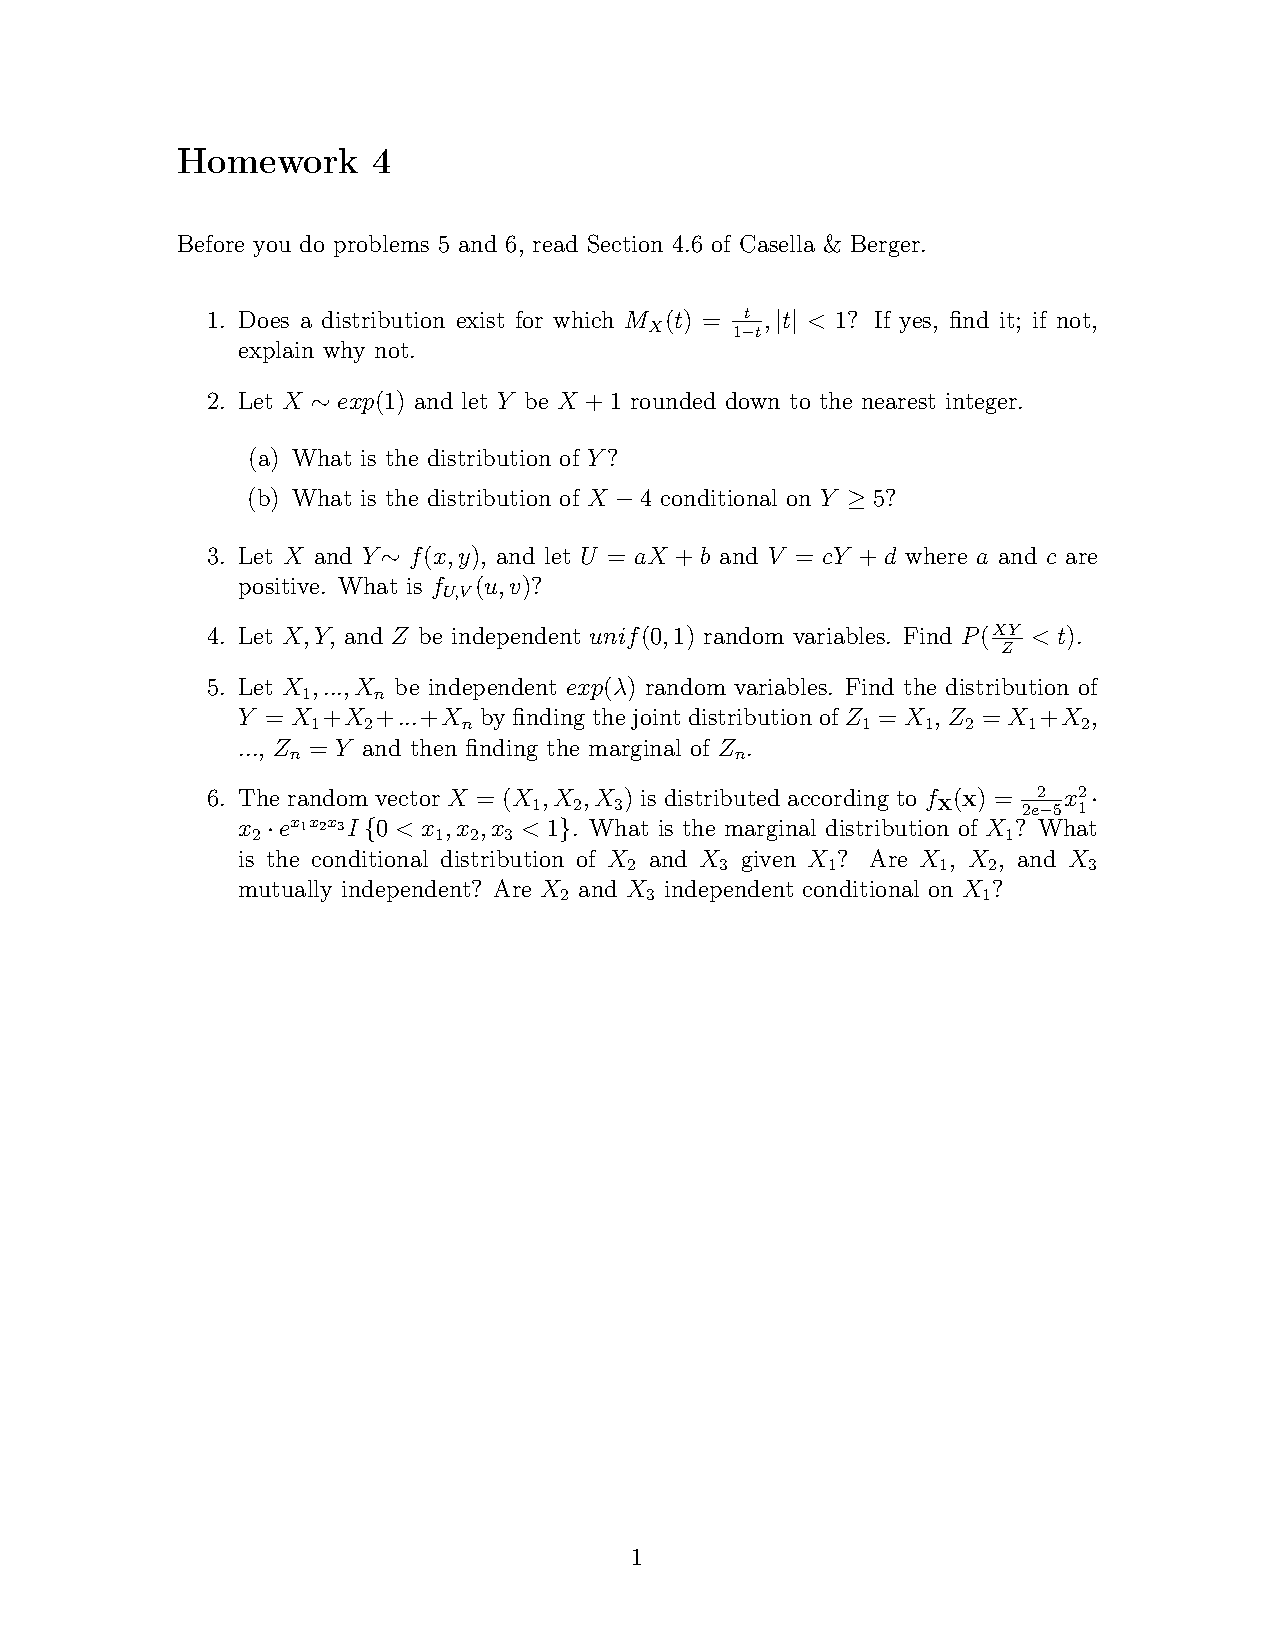
\includepdf[pages=-]{HW_4.pdf}
\maketitle

\begin{enumerate}
    \item $M_X(t)$ is not a moment generating function of some random variable. 
    Becuase for every $X$, $M_X(t) = \mathbb{E}[e^{tX}]$, so $M_X(0)$ will always be $1$. However here $M_X(0) = 0$, a contradiction.

    \item 
    \begin{enumerate}[(a)]
        \item
        $Y$ is an integer valued random variable from $1$ to $\infty$. And its pmf is 
        $$\textbf{P}(Y = k) = \textbf{P}(k-\frac{1}{2} \le X+1 < k+\frac{1}{2}) = 
            \begin{cases}
                1 - e^{-\frac{1}{2}} & \text{if}\ k = 1\\
                (e^{\frac{3}{2}} - e^{\frac{1}{2}})e^{-k} & \text{if}\ k > 1
            \end{cases} $$

        \item
        We derive the cdf of $X - 4$ condition on $Y \ge 5$.
        \begin{eqnarray}
             \prob{X - 4 \le t | Y \ge 5} &=& \frac{\prob{X - 4 \le t ; Y \ge 5}}{\prob{Y \ge 5}} \\
                                          &=& \frac{\prob{X - 4 \le t ; X + 1 \ge 4.5}}{\prob{X + 1 \ge 4.5}} \\             
                                          &=& \frac{\prob{3.5 \le X \le 4 + t}}{\prob{X \ge 3.5}} \\
                                          &=& 1 - e^{-(t + \frac{1}{2})}
        \end{eqnarray}
        where $t > -\frac{1}{2}$.
    \end{enumerate}

    \item
    Then we have $X = \frac{1}{a} (U - b)$, $\frac{1}{c} (V - d)$ and $|\frac{\partial (X, Y)}{\partial (U, V)}| = \frac{1}{ac}$.
    Therefore 
    $$f_{U,V}(u,v) = \frac{1}{ac} f(\frac{1}{a} (u - b) , \frac{1}{c} (v - d))$$

    \item 
    We have: 
       $$\prob{\frac{XY}{Z} < t} = \iiint_{xy<tz;\ 0<x,y,z<1} 1\ d x d y d z $$
    Of course $t$ should be bigger than $0$. If $t \le 1$, we have:
    \begin{eqnarray}
        \prob{\frac{XY}{Z} < t} &=& \iiint_{xy<tz;\ 0<x,y,z<1} 1\ d x d y d z \\
                                &=& \int_0^1 dz \int_0^1 dy \int_0^{\min(1,\frac{tz}{y})} 1\ dx \\
                                &=& \int_0^1 dz (\int_0^{tz} + \int_{tz}^1) \min(1,\frac{tz}{y}) dy \\
                                &=& \int_0^1 (tz - tz\log{tz}) dz \\
                                &=& \frac{3 t}{4} - \frac{t}{2}\log{t}
    \end{eqnarray}
    And if $t > 1$, we have:
    \begin{eqnarray}
        \prob{\frac{XY}{Z} < t} &=& \iiint_{xy<tz;\ 0<x,y,z<1} 1\ d x d y d z \\
                                &=& \int_0^1 dz \int_0^1 dy \int_0^{\min(1,\frac{tz}{y})} 1\ dx \\
                                &=& \int_0^1 dz \int_0^1 \min(1,\frac{tz}{y}) dy \\
                                &=& (\int_0^{\frac{1}{t}} + \int_{\frac{1}{t}}^1) (\int_0^1 \min(1,\frac{tz}{y}) dy) dz \\
                                &=& \int_{\frac{1}{t}}^1 1\ dz + \int_0^{\frac{1}{t}} dz ((\int_0^{tz} + \int_{tz}^1) \min(1,\frac{tz}{y}) dy) \\
                                &=& (1 - \frac{1}{t}) + \frac{3}{4t} = 1 - \frac{1}{4t}
    \end{eqnarray}
    Therefore:
    $$ \prob{\frac{XY}{Z} < t} = \begin{cases}
                                    \frac{3 t}{4} - \frac{t}{2}\log{t} & 0< t \le 1 \\
                                    1 - \frac{1}{4t} & t > 1  
                                \end{cases}$$

    \item
    The joint density of $X_1, X_2,\cdots, X_n$ is $f(x_1,x_2,\cdots,x_n) = \lambda^n e^{-\lambda \sum_{i=1}^n x_i} \bm{1}_{\{\text{all}\ x_i > 0\}}$.
    By using the transformation as in the question, we have 
    $$|\frac{\partial(X_1,X_2,\cdots,X_n)}{\partial(Z_1,Z_2,\cdots,Z_n)}| = |\frac{\partial(Z_1,Z_2,\cdots,Z_n)}{\partial(X_1,X_2,\cdots,X_n)}|^{-1} = 1$$
    So we have the joint density of $Z_1,Z_2,\cdots,Z_n$ is 
    $$f_{Z_1,Z_2,\cdots,Z_n}(z_1,z_2,\cdots,z_n) = \lambda^n e^{-\lambda z_n} \bm{1}_{\{z_1 < z_2 < \cdots < z_n\}}$$
    Then marginalizing on $Z_n$, we get:
    $$f_{Z_n}(z_n) = \int_0^{z_n} dz_{n-1} \int_0^{z_{n-1}} dz_{n-2} \cdots \int_0^{z_2} \lambda^n e^{-\lambda z_n} dz_1 = \lambda^n \frac{z_n^{n-1}}{(n-1)!} e^{-\lambda z_n} \bm{1}_{z_n>0}$$
    Therefore the pdf of $Y$ is $f_Y(y) = \frac{\lambda^n y^{n-1}}{(n-1)!} e^{-\lambda y} \bm{1}_{y>0}$.

    \item
    We have:
    \begin{eqnarray}
        f_{X_1}(x_1) &=& \frac{2}{2e-5} x_1 \int_0^1 dx_2\int_0^1 x_1 x_2 e^{x_1 x_2 x_3}dx_3 \\
                     &=& \frac{2}{2e-5} \int_0^1 x_1 e^{x_1 x_2} - x_1 dx_2 = \frac{2}{2e-5} (e^{x_1} - x_1 -1)         
    \end{eqnarray}
    where $0< x_1 <1$.
    Then the conditional density:
    $$f_{X_2,X_3}(x_2,x_3 | x_1) = \frac{x_1^2}{e^{x_1}-x_1-1} x_2 e^{x_1 x_2 x_3} \bm{1}_{0<x_2,x_3<1}$$

    $X_1,X_2,X_3$ are not mutually independent, because $e^{x_1 x_2 x_3}$ can not be factorized.

    Also $X_2$ and $X_3$ are not independent conditional on $X_1$, because $e^{x_1 x_2 x_3}$ can not be factorized.

\end{enumerate}

\end{document}